\AddToShipoutPictureBG*{
    \AtPageLowerLeft{
        
\includegraphics[width=\paperwidth,height=\paperheight]{chapters/chapter5.jpg}
    }
}

\decorate{相守}

\pagestyle{empty}

\Large
\begin{center}
    \vspace*{1.5cm}
    \color{white}
    {
    樱花停驻你衣襟时 \par \vspace*{0.4cm}
    我们正走过三月的桥 \par   \vspace*{0.4cm}
    柳絮在风中签下白首的约 \par\vspace*{0.4cm}
    溪流搬运着光的碎片 \par\vspace*{0.4cm}
    将两个倒影 \par\vspace*{0.4cm}
    熔铸成同一道波浪 \par\vspace*{0.4cm}
    燕子在檐下重复 \par\vspace*{0.4cm}
    去年衔来的韵脚 \par \vspace*{0.4cm}
    桃树把花瓣数进我们合拢的掌纹 \par \vspace*{0.4cm}
    当薄雾散去 \par \vspace*{0.4cm}
    整个春天都在证明 \par \vspace*{0.4cm}
    相守是永不凋零的节气
    }
    \vfill 
    \makefoot
\end{center}

\card{covers/cover22.jpg}{V}{珍惜当下}{Value this moment}

\setstyle{Value this moment}

\subtitle{初遇家门——你的到来}

\large
\begin{spacing}{2}
    你来深圳，专程来见我和我的家人。那天清晨，我赶忙去火车站接你，快到家的时候你买了很多很多的礼物。
    到家的时候阳光透过窗户洒在餐桌上，你静静坐在旁边。
    
    我脚刚受伤，行动略显迟缓，你轻轻为我擦拭脚上的疲惫和微微的红肿。动作小心而温柔，像在照顾一件易碎的宝物。我的心猛地一紧，有些感动得说不出话，眼角却忍不住湿润。

    这一刻，不只是脚上的疼痛被你抚平，更是心里的温度被悄悄升起。你的在意、你的体贴，让我明白：爱情的细节，有时候就在最平凡的动作里静静发生。

    \bottomtext{“你的温柔成为最深的温暖。”}
\end{spacing}

\card{covers/cover23.jpg}{W}{走这条路}{Walk this path}

\setstyle{Walk this path}

\subtitle{大梅沙——海风签名式}

\large
\begin{spacing}{2}
    大梅沙的海风裹挟着咸涩的气息扑面而来，温柔地吹散了城市里积攒的喧嚣，也吹起了我心底如海浪般轻盈的欢快。
    我们踩在细软的金色沙滩上，湿润的砂粒在脚趾间流动，带着微凉的触感。海浪不知疲倦地轻吻着岸边，
    发出舒缓的哗哗声，像一位耐心的公证人，正在为我们的到来签下独一无二的印记。

    你在前面小跑着，沙滩上留下一串浅浅的脚印，清脆的笑声被海风托起，飘向蔚蓝的远方。我紧随其后，
    在我们的脚印旁留下并行的痕迹。偶尔，我们会停下奔跑的脚步，蹲下身，
    用手指在潮湿的沙面上写下一些标记，画上可爱的涂鸦，或是勾勒出小小的心形图案。然后相视一笑，
    任由涌上的潮水为我们的创作"盖章认证"。每一次低头，看着海浪将我们刚刚写下的名字温柔地抹平，
    我都忍不住笑出声来——也许这就是我们最独特的"签名方式"，短暂得只存在于一个浪起浪落之间，
    却又永恒地烙印在彼此的记忆画布上。

    午后的阳光穿过云层，洒下恰到好处的温暖。海面泛起粼粼波光，像无数蓝色碎钻在跳跃闪烁。
    我们的身影在沙滩上被拉得细长，时而分开，时而交叠，仿佛在演绎一场无声的双人舞。海风调皮地撩起你的发丝，
    也轻轻拨动着我的心弦。那一刻，时间仿佛被施了魔法，静止在这片蔚蓝的天地间——耳边只有海浪的吟唱，
    脚下只有砂粒的柔软，而我的世界里，只有你在身边的温暖。

    \begin{figure}[!htbp]
        \centering
        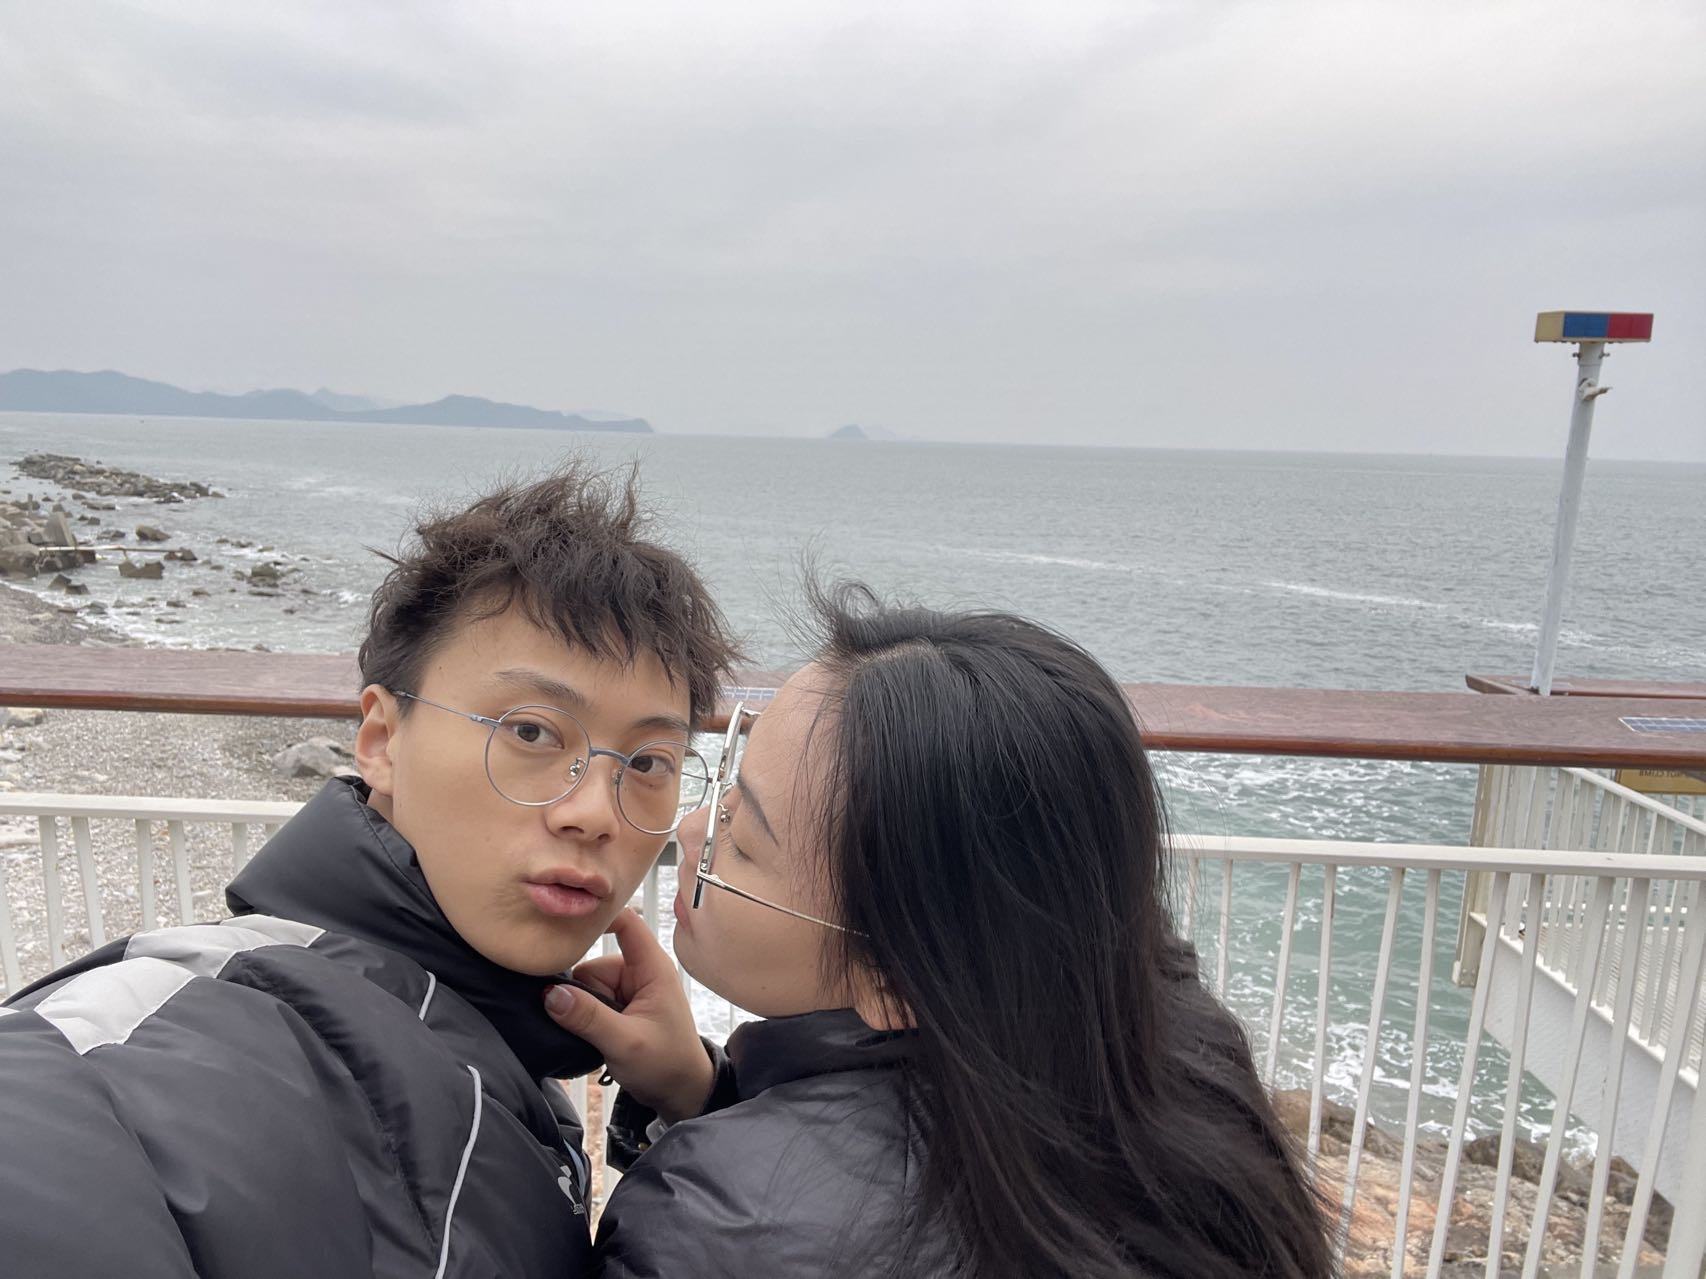
\includegraphics[width=0.8\textwidth]{figures/articles/04-1.jpg}
        \caption*{\small{2024年12月23日，大梅沙海边散步}}
    \end{figure}

    \bottomtext{“海风是我们的签名，沙滩是我们的画布，记忆在每一次潮起潮落中留下痕迹。”}
\end{spacing}

\card{covers/cover24.jpg}{X}{加大号的爱}{XL love}

\setstyle{XL love}

\subtitle{我的21岁生日——二十一岁光年}

\large
\begin{spacing}{2}
    那天，是我21岁的生日。吉安的阳光温暖而柔和，仿佛为这一年最特别的日子镀上了一层金色光晕。
    你捧着精心挑选的蛋糕，我在你微笑的目光里感受到了21岁的温度：既有成长的重量，
    也有被珍惜的幸福。生日不仅是岁数的标记，更像一次光年的旅行，而你，
    就是这段光年里最温暖的风景。

    \begin{figure}[!htbp]
        \centering
        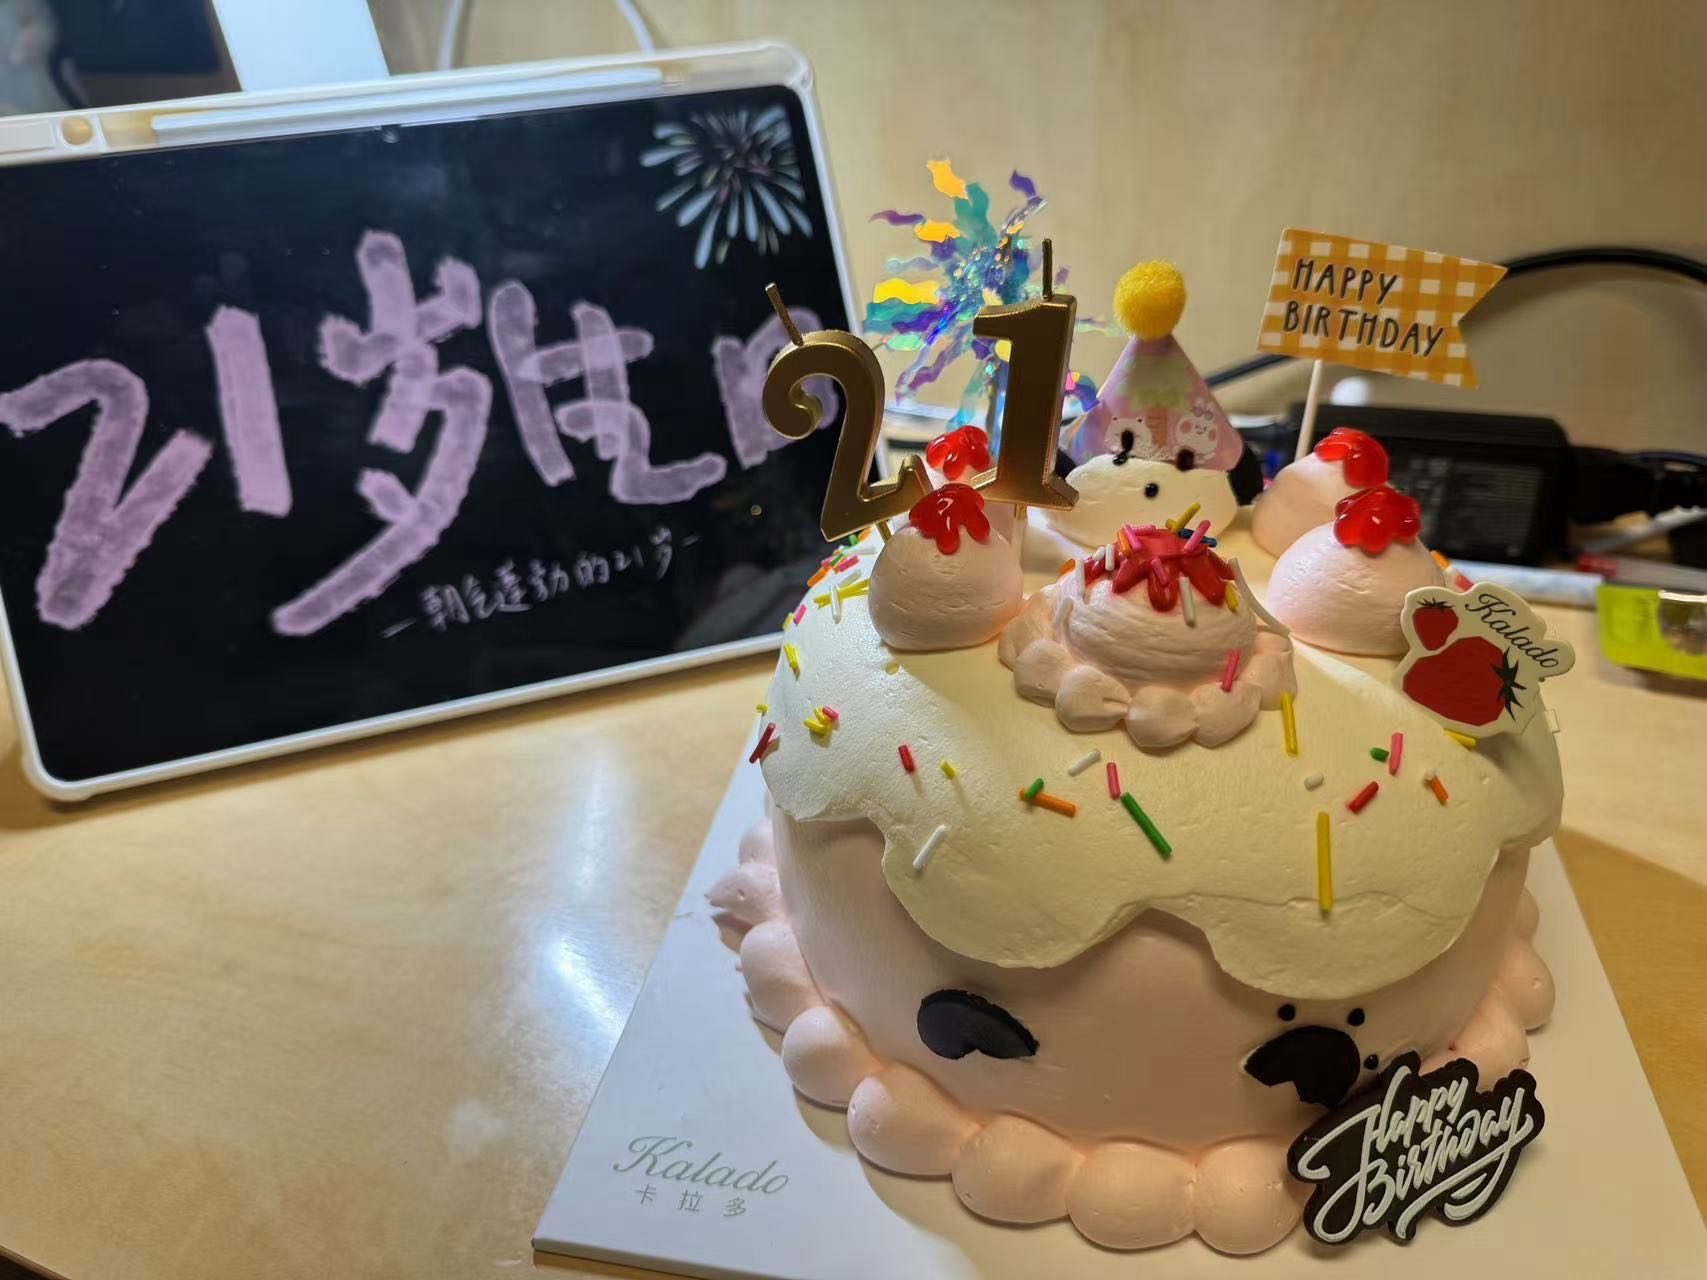
\includegraphics[width=0.6\textwidth]{figures/articles/04-3.jpg}
        \caption*{\small{2025年1月14日，我的21岁生日}}
    \end{figure}

    \bottomtext{“二十一岁的光年里，你是我最亮的星。”}
\end{spacing}

\card{covers/cover25.jpg}{Y}{渴望你的存在}{Yearn for your presence}

\setstyle{Yearn for your presence}

\subtitle{专升本考试——季风远征记}


\vspace*{2cm}
\large
\begin{bbox}
    \begin{center}
        至于这场专升本考试 \par \vspace*{0.5cm}
        只是你最后插在它身上的旗帜 \par \vspace*{0.5cm}
        你已经成功了 \par \vspace*{0.5cm}
        我祝贺你 \par \vspace*{0.5cm}
        不止是你度过了难关 \par \vspace*{0.5cm}
        更因为世界上又多了一个勇敢又善良的大人
    \end{center}
\end{bbox}

\bottomtext{“在考试的远征里，我是你最温暖的后盾。”}

\card{covers/cover26.jpg}{Z}{对你狂热}{zeal for you}

\setstyle{zeal for you}

\subtitle{香港之行——维港漫游指南}

\large
\begin{spacing}{2}
    那天的香港，天色澄净，阳光被海风打磨得温柔又明亮。我们从地铁站出来，街头的英文招牌和叮当作响的电车声交织在一起，像是一首属于这座城市的老歌。空气里有海的味道，也有夏天特有的明快。

    我们穿过弥敦道的人潮，沿着中环一路走向维港。一路上我们逛了万宁、sasa等好多店铺，你说你想吃富豪雪糕，我看着你认真的神情，不由得我们的距离也近了。

    午后，我们走进K11 MUSEA。那是一个被设计感包裹的空间，光线从玻璃穹顶洒下，照在艺术装置与海景交织的每个角落。我们一边逛，一边感叹这里的精致与浪漫——在每一个不经意的转角，都能遇见一点点生活的惊喜。

    傍晚，我们登上天星小轮。海风扑面而来，带着一点咸味。你坐在座位上，长发被风扬起，我在你身侧，看对岸的高楼被夕阳染成金色。船身在水面轻轻摇晃，像是时间也在这短短几分钟里放慢了脚步。  

    登岸后，我们顺着维港的长廊走到摩天轮。天边的霞光正好褪去，天空从浅蓝转为温柔的灰粉。我们坐进透明的舱里，城市在脚下缓缓展开——维港的水面、街头的车流、还有那一整片被夕阳点亮的屋顶。你坐在我对面，我很想轻声说：“真希望这一刻能久一点。”心里想，这一刻，已经足够久。

    \begin{figure}[!htbp]
        \centering
        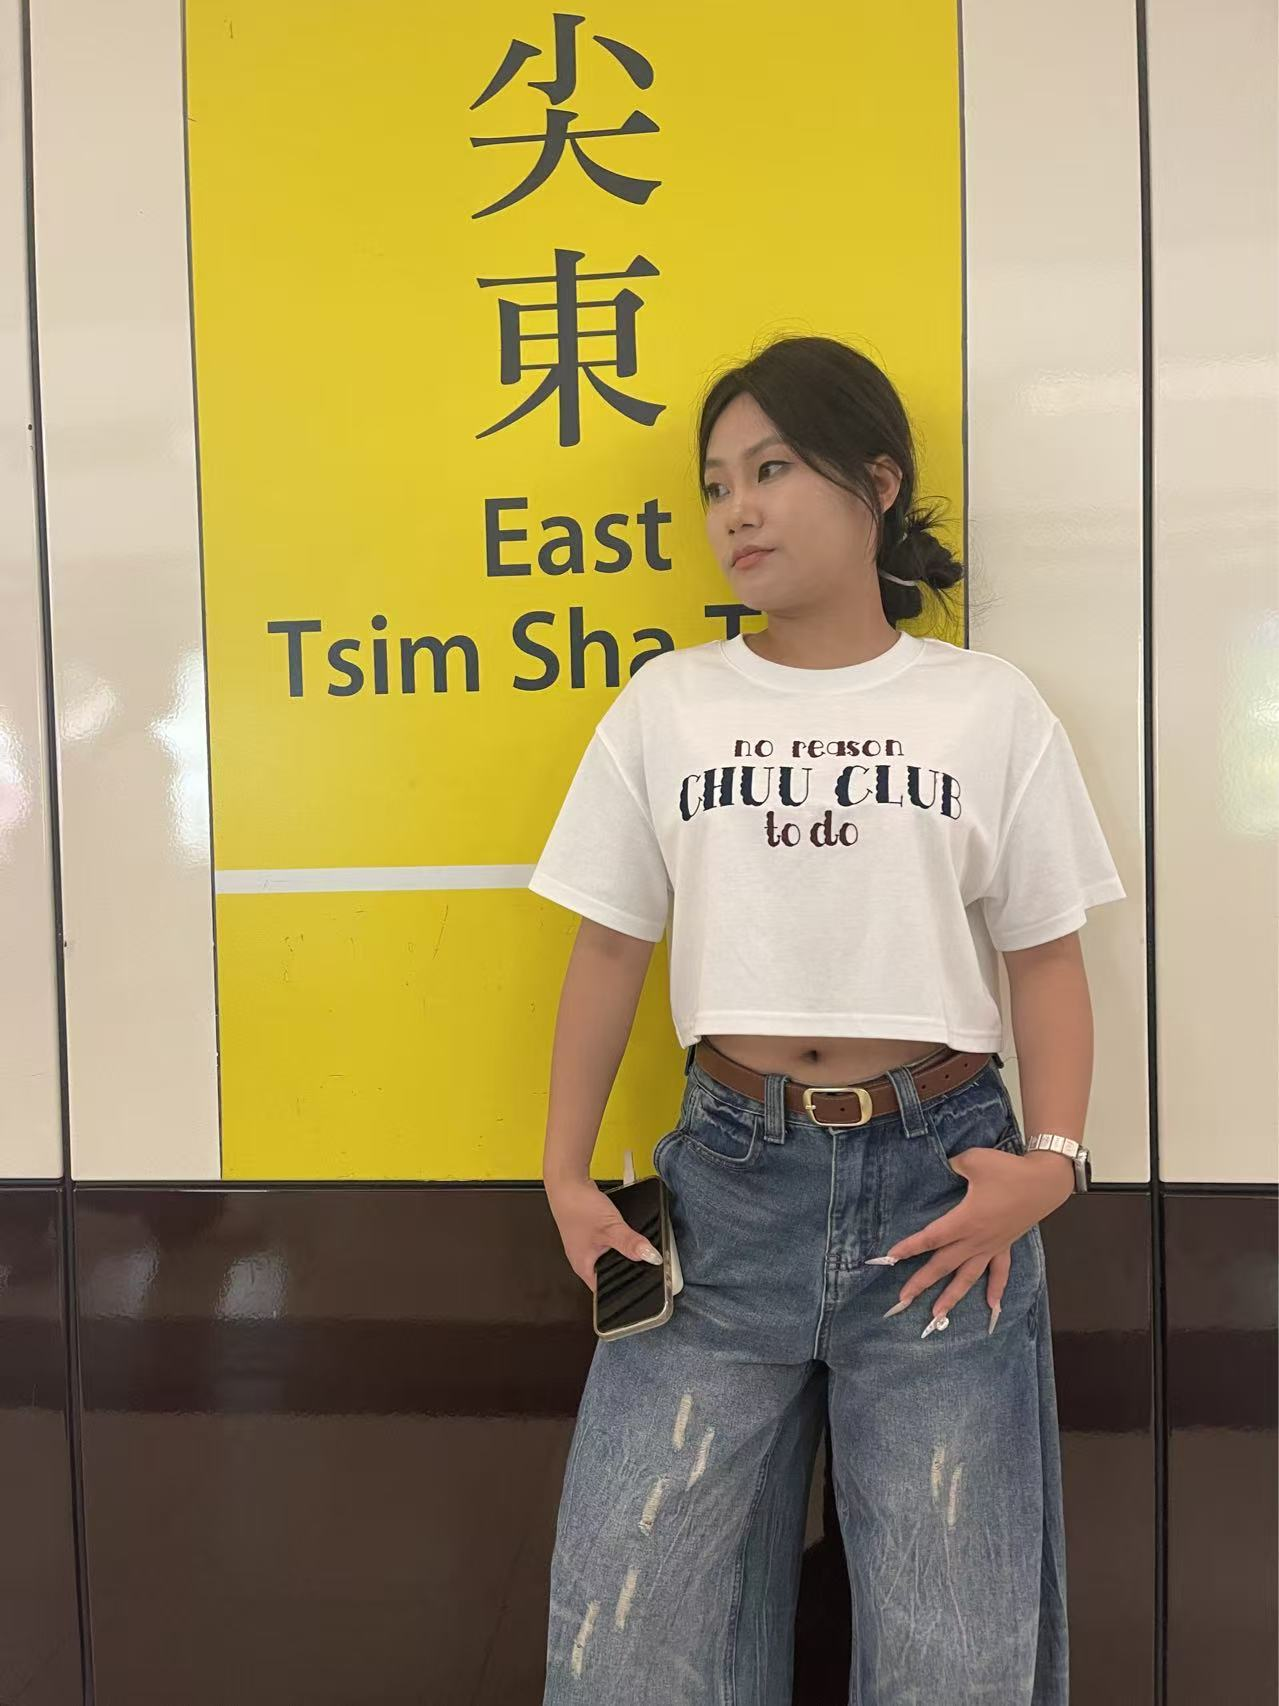
\includegraphics[width=0.5\textwidth]{figures/articles/04-4.jpg}
        \caption*{\small{2025年8月8日于香港}}
    \end{figure}

    \bottomtext{“我们在海风与人潮中穿行，把白昼写成一首慢歌。”}
\end{spacing}

\clearpage
